\documentclass[11pt,a4paper]{article}
\usepackage[utf8]{inputenc}
\usepackage[spanish]{babel}
\usepackage{graphicx}
\usepackage{geometry}
\geometry{top=2.5cm, bottom=2.5cm, left=2.5cm, right=2.5cm}
\usepackage{hyperref}
\usepackage{titlesec}

\title{\textbf{Manual de Usuario Corporativo: Operaciones Integradas en Odoo ERP}}
\author{}
\date{}

\begin{document}

\maketitle
\tableofcontents
\newpage

\section{Módulo de Contactos (Fichas de Clientes)}
Este módulo sirve para guardar y organizar los datos de tus clientes (personas o empresas). Mantenerlo al día evita problemas con la SUNAT en facturas electrónicas.

\subsection{Ver Listado de Clientes (Leer)}
En tu pantalla de inicio de Odoo, busca el icono que dice \textbf{Contactos} y haz clic sobre él. Verás una pantalla con tarjetas de los clientes creados.

\begin{center}
    \makebox[\textwidth][c]{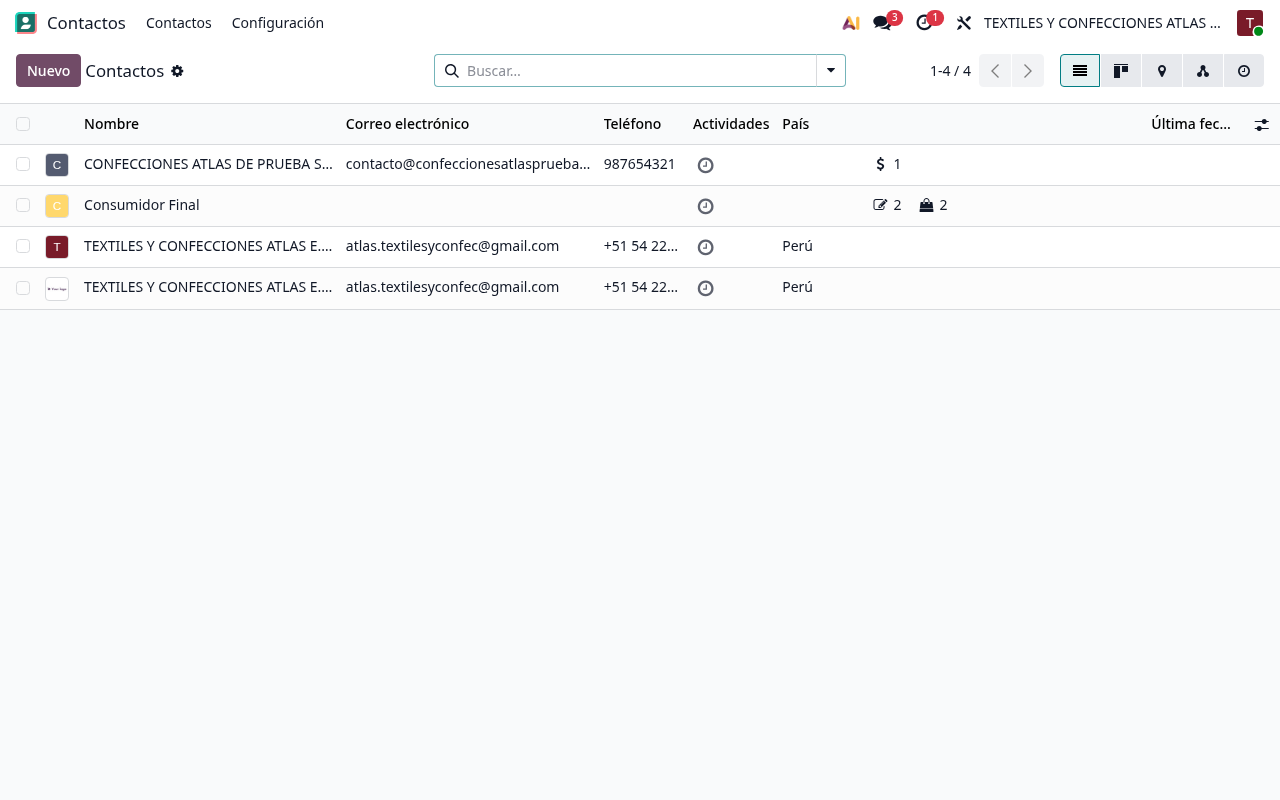
\includegraphics[width=1.15\textwidth]{images/contactos_crud_read.png}}
\end{center}

\subsection{¿Cómo Buscar Clientes rápidamente?}
\begin{enumerate}
    \item En la parte superior derecha de la pantalla de Contactos verás una barra con una pequeña lupa.
    \item Haz clic dentro de esta barra de búsqueda.
    \item Escribe lo que buscas (por ejemplo: el nombre de la empresa, el RUC o el teléfono).
    \item Presiona \textbf{Enter} y la pantalla ocultará temporalmente a los demás clientes, mostrando solo el que escribiste.
\end{enumerate}

\begin{center}
    \makebox[\textwidth][c]{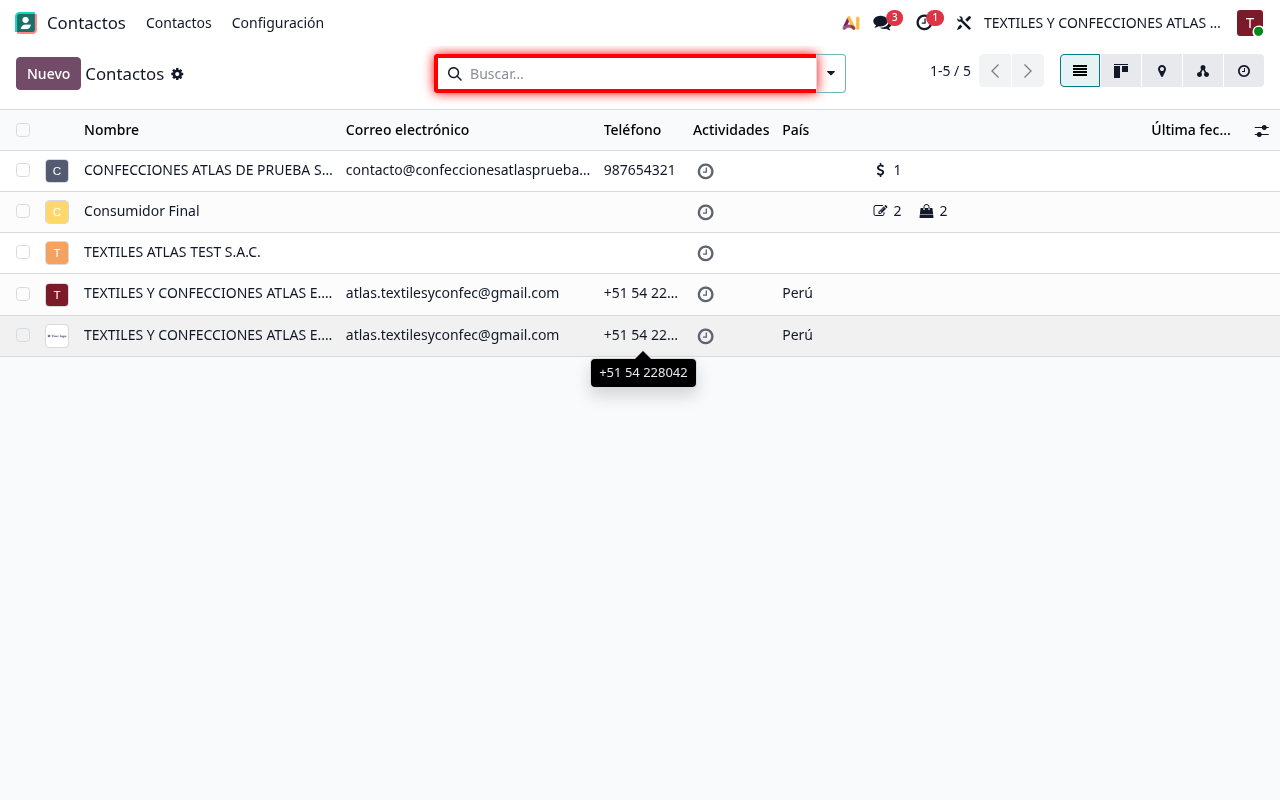
\includegraphics[width=1.15\textwidth]{images/contactos_busqueda_filtros.png}}
\end{center}
\textit{Figura 1.1: Barra de búsqueda superior para encontrar clientes por nombre, RUC o datos de contacto.}

\subsection{Uso de Filtros y Agrupadores (Ordenar a tus clientes)}
Para segmentar a tu cliente rápidamente sin tener que buscar uno por uno:
\begin{enumerate}
    \item Haz clic en el botón \textbf{Filtros} que está justo debajo de la barra de búsqueda.
    \begin{itemize}
        \item \textit{Ejemplo de uso:} Si solo quieres ver a las empresas registradas (personas jurídicas) y ocultar a las personas naturales, selecciona el filtro \textbf{Compañías}.
    \end{itemize}
    \item Haz clic en \textbf{Agrupar por}:
    \begin{itemize}
        \item \textit{Ejemplo de uso:} Si tienes clientes en distintos departamentos del Perú y deseas ordenarlos visualmente por su ubicación, haz clic en \textbf{País/Estado} o \textbf{Ciudad}. Odoo los dividirá de forma ordenada en bloques agrupados.
    \end{itemize}
\end{enumerate}

\subsection{Cambiar de Vistas (Tarjetas vs. Tablas)}
En la parte superior derecha verás tres pequeños botones para cambiar la forma en que se muestra la información:
\begin{itemize}
    \item \textbf{Vista Kanban (Tarjetas):} Muestra cada cliente en un recuadro individual con su foto y datos rápidos.
    \item \textbf{Vista Lista (Tabla):} Muestra a los clientes en una tabla compacta como una hoja de Excel. Es la mejor opción cuando necesitas comparar datos rápidamente.
    \item \textbf{Vista Mapa:} Muestra la ubicación geográfica del cliente en Google Maps.
\end{itemize}

\begin{center}
    \makebox[\textwidth][c]{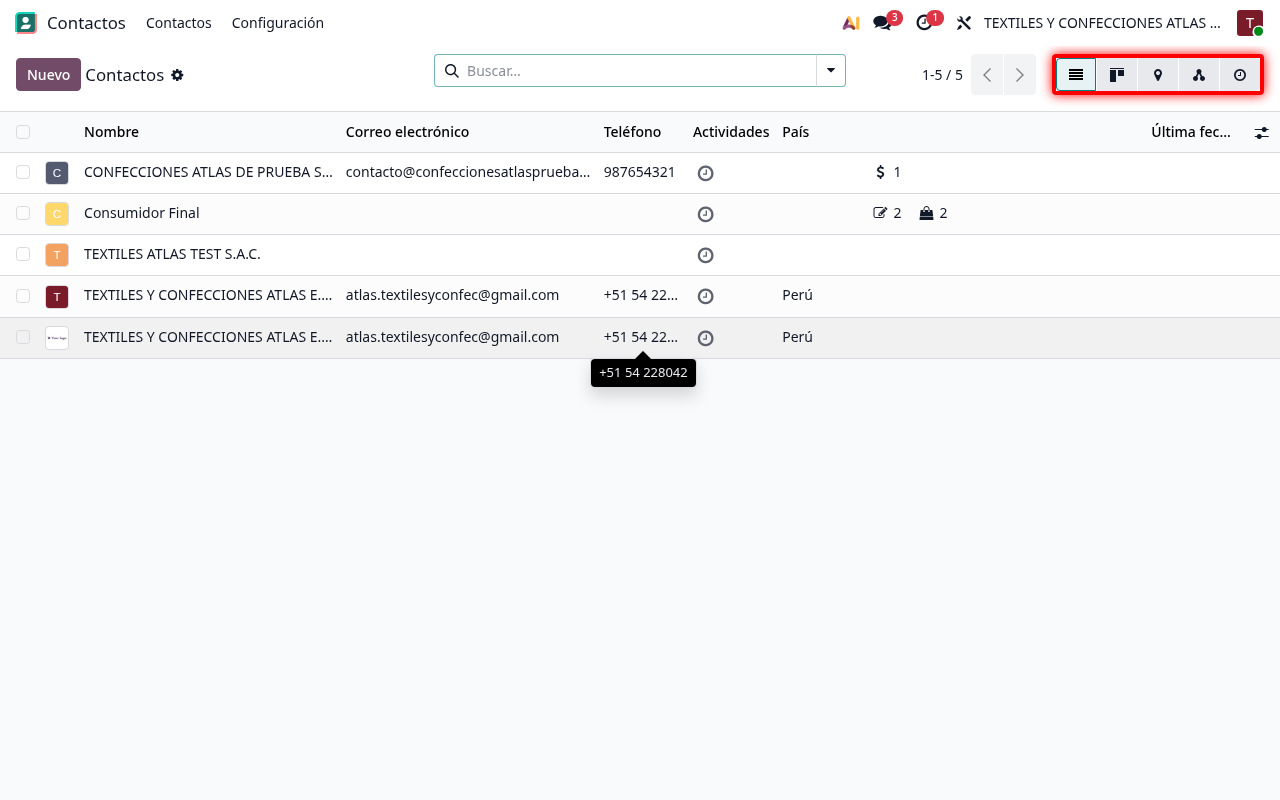
\includegraphics[width=1.15\textwidth]{images/contactos_cambio_vistas.png}}
\end{center}
\textit{Figura 1.2: Botones para alternar entre las vistas Kanban (tarjetas) y Lista (tabla) en Odoo.}

\subsection{Hacer clic en Crear Nuevo Cliente}
\begin{enumerate}
    \item Ubica el botón \textbf{Nuevo} en la parte superior izquierda (enmarcado en rojo).
    \item Haz clic sobre él.
\end{enumerate}

\begin{center}
    \makebox[\textwidth][c]{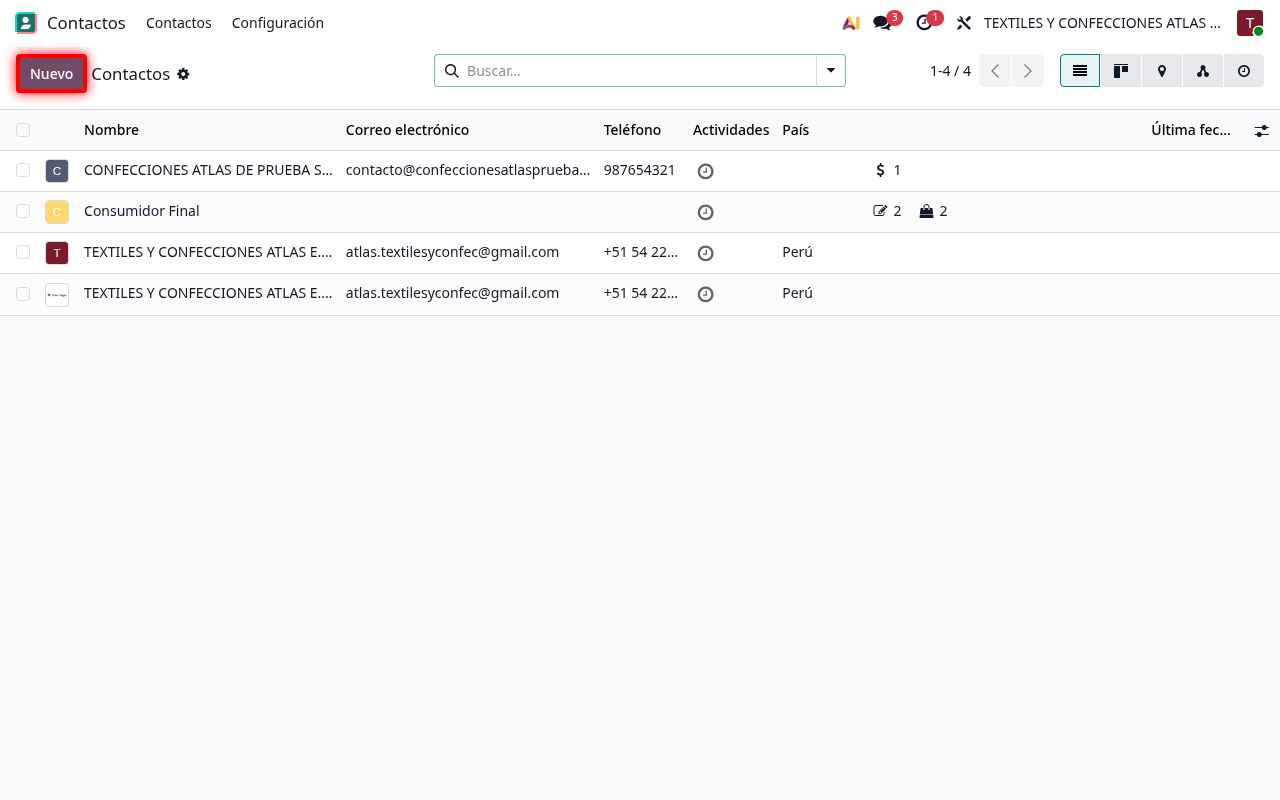
\includegraphics[width=1.15\textwidth]{images/contactos_crud_click_create.png}}
\end{center}

\subsection{Rellenar la Ficha del Cliente (Ejemplo Práctico)}
\begin{enumerate}
    \item En el campo \textbf{Nombre}, escribe el nombre del cliente o empresa (Ejemplo: \textit{TEXTILES ATLAS TEST S.A.C.}).
    \item En \textbf{Identificación Fiscal}, selecciona \textbf{RUC} o \textbf{DNI}.
    \item En el campo \textbf{Número de Identificación}, escribe el número correspondiente (Ejemplo: \textit{20123456789}).
    \item Haz clic en \textbf{Guardar} (el icono de la nube en la parte superior izquierda).
\end{enumerate}

\begin{center}
    \makebox[\textwidth][c]{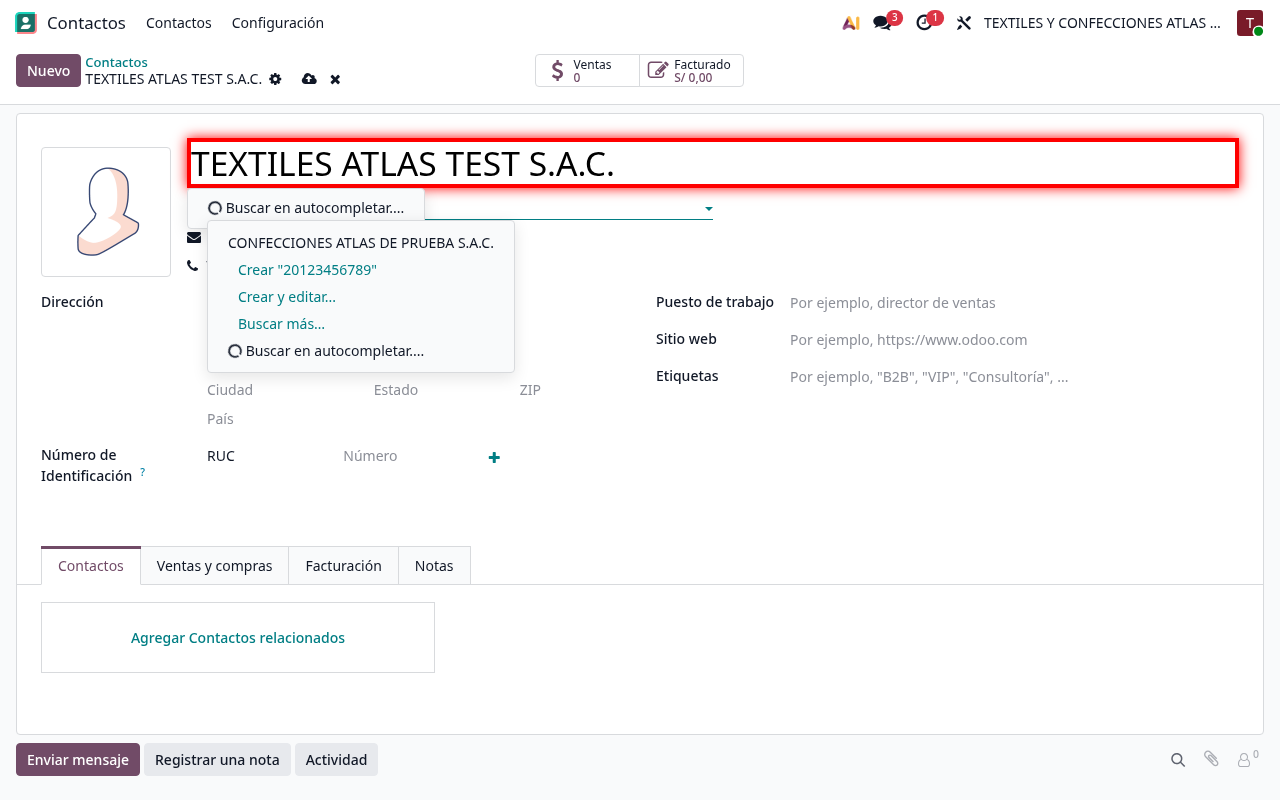
\includegraphics[width=1.15\textwidth]{images/contactos_crud_fill_name.png}}
\end{center}
\begin{center}
    \makebox[\textwidth][c]{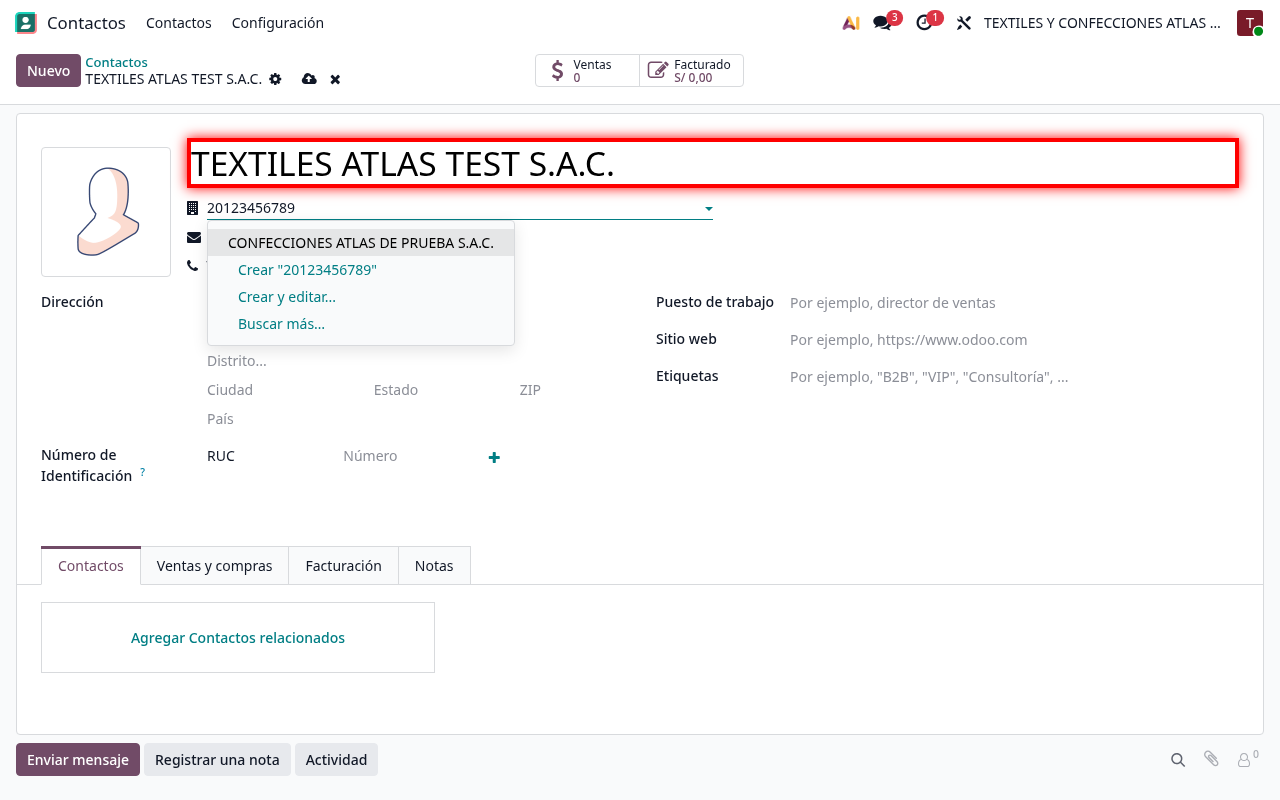
\includegraphics[width=1.15\textwidth]{images/contactos_crud_fill_vat.png}}
\end{center}
\newpage

\section{El Chatter: El Historial y Centro de Mensajería de Odoo}
El \textbf{Chatter} (sección de comunicación) es una de las herramientas más importantes de Odoo. Se encuentra en el lateral derecho de \textbf{todas las fichas} de Odoo (Contactos, Ventas, Inventario, etc.).

Sirve como una bitácora o cuaderno de notas donde se registra todo lo que pasa con ese cliente para que cualquier trabajador del negocio esté enterado.

\begin{center}
    \makebox[\textwidth][c]{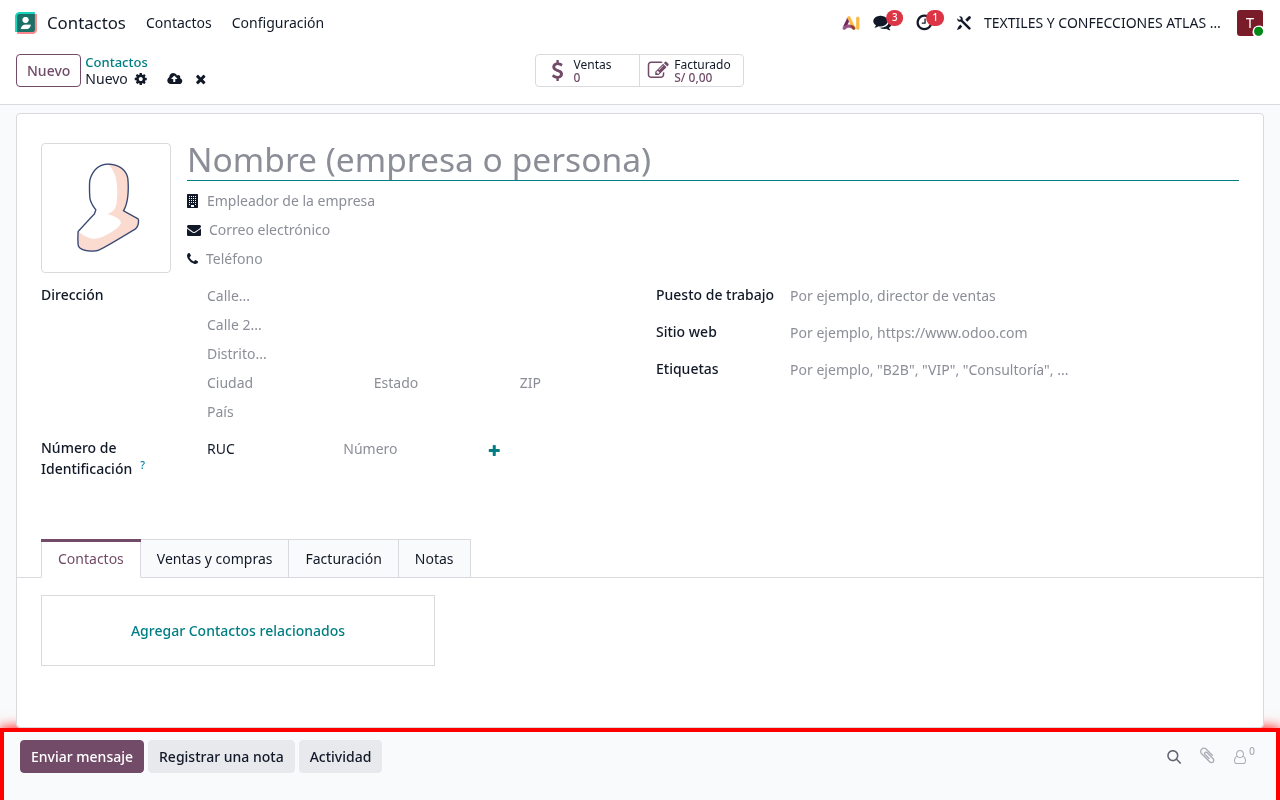
\includegraphics[width=1.15\textwidth]{images/contactos_chatter.png}}
\end{center}
\textit{Figura 2.1: Panel del Chatter en el costado derecho de la ficha del contacto.}

\subsection{Enviar Mensaje (Comunicación Directa)}
\begin{itemize}
    \item \textbf{¿Para qué sirve?:} Para enviar correos electrónicos al cliente directamente desde Odoo, sin abrir Outlook o Gmail.
    \item \textbf{¿Cómo se hace?:}
    \begin{enumerate}
        \item Haz clic en \textbf{Enviar mensaje}.
        \item Escribe tu texto.
        \item Haz clic en \textbf{Enviar}. El cliente recibirá el correo y si responde, su respuesta aparecerá aquí mismo.
    \end{enumerate}
\end{itemize}

\subsection{Poner Nota (Bitácora Interna)}
\begin{itemize}
    \item \textbf{¿Para qué sirve?:} Para apuntar cosas importantes sobre el cliente que solo tus compañeros de trabajo deben ver (el cliente NO recibe correos de estas notas).
    \item \textbf{¿Cómo se hace?:}
    \begin{enumerate}
        \item Haz clic en \textbf{Poner nota}.
        \item Escribe datos útiles como: \textit{"Este cliente prefiere recibir cotizaciones los martes"}.
        \item Haz clic en \textbf{Registrar nota}.
    \end{enumerate}
\end{itemize}

\subsection{Planificar Actividad (Recordatorios)}
\begin{itemize}
    \item \textbf{¿Para qué sirve?:} Para que Odoo te recuerde hacer una tarea con el cliente en una fecha específica.
    \item \textbf{¿Cómo se hace?:}
    \begin{enumerate}
        \item Haz clic en \textbf{Planificar actividad} (icono de reloj).
        \item Selecciona el tipo de actividad (ej. \textit{Llamar}).
        \item Coloca la fecha límite y una descripción rápida.
        \item Haz clic en \textbf{Planificar}. Odoo te recordará la tarea el día acordado.
    \end{enumerate}
\end{itemize}
\newpage

\section{Módulo de Inventario (Gestión de Productos)}
Aquí podrás ver qué prendas tienes disponibles y añadir nuevas al catálogo de la tienda.

\subsection{Ver Catálogo de Productos (Leer)}
\begin{enumerate}
    \item Haz clic en el botón de \textbf{Inventario} en el menú de aplicaciones de Odoo.
    \item Selecciona \textbf{Productos} en el menú de arriba.
\end{enumerate}

\begin{center}
    \makebox[\textwidth][c]{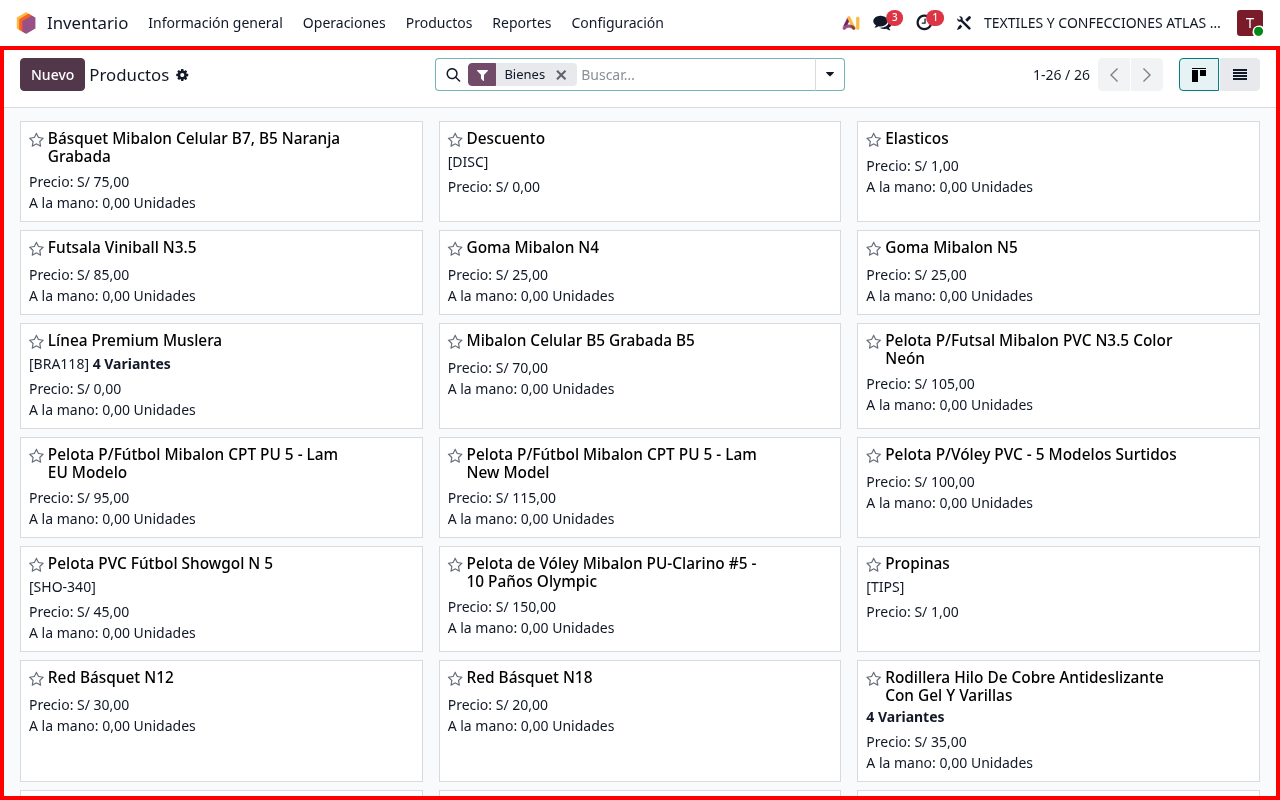
\includegraphics[width=1.15\textwidth]{images/inventario_crud_read.png}}
\end{center}

\subsection{Crear un Producto Nuevo (Ejemplo Práctico)}
\begin{enumerate}
    \item Haz clic en el botón \textbf{Nuevo} en la esquina superior izquierda.
    \item Completa los campos solicitados:
    \begin{itemize}
        \item \textbf{Nombre del Producto:} Escribe el nombre de la prenda (Ejemplo: \textit{Casaca Térmica Impermeable Talla L}).
        \item \textbf{Tipo de Producto:} Selecciona \textbf{Almacenable} para llevar control de unidades.
        \item \textbf{Precio de Venta:} Escribe el precio en Soles (Ejemplo: \textit{120.00}).
    \end{itemize}
    \item Presiona \textbf{Guardar}.
\end{enumerate}

\begin{center}
    \makebox[\textwidth][c]{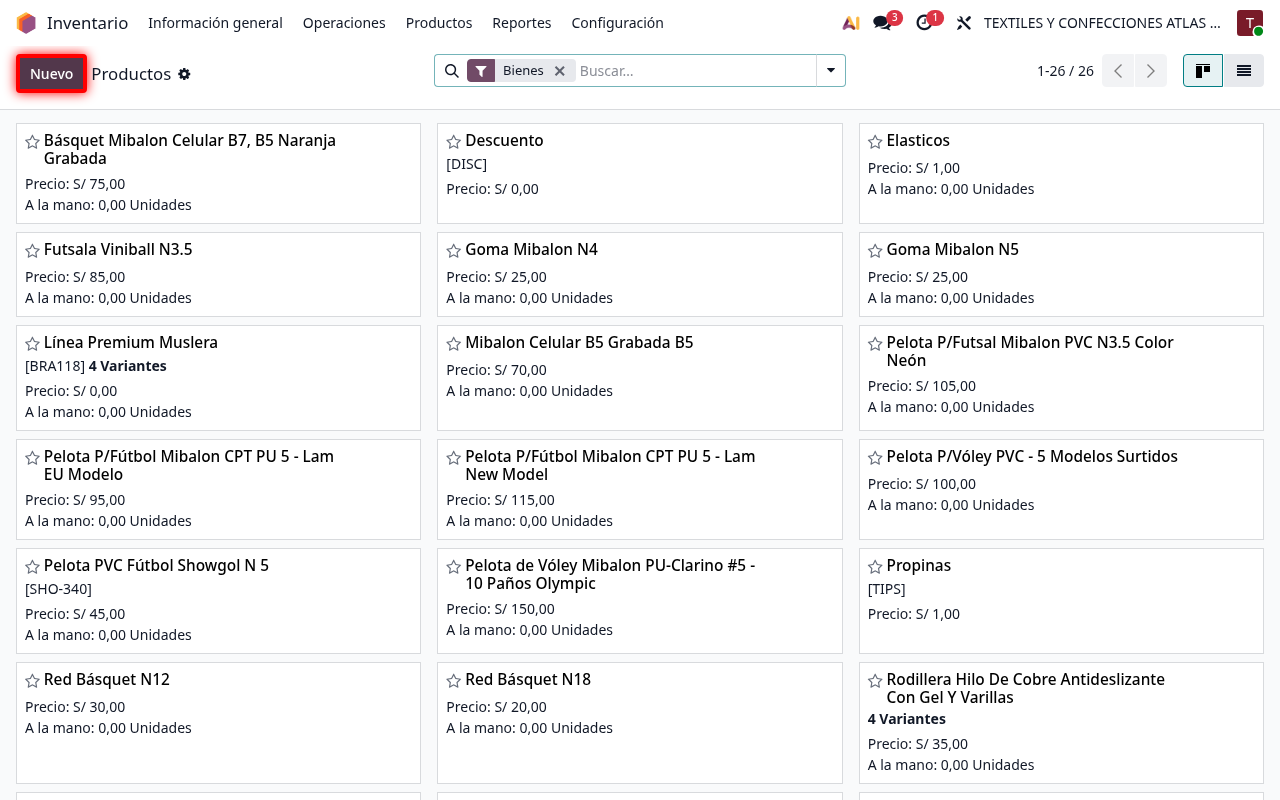
\includegraphics[width=1.15\textwidth]{images/inventario_crud_click_create.png}}
\end{center}
\begin{center}
    \makebox[\textwidth][c]{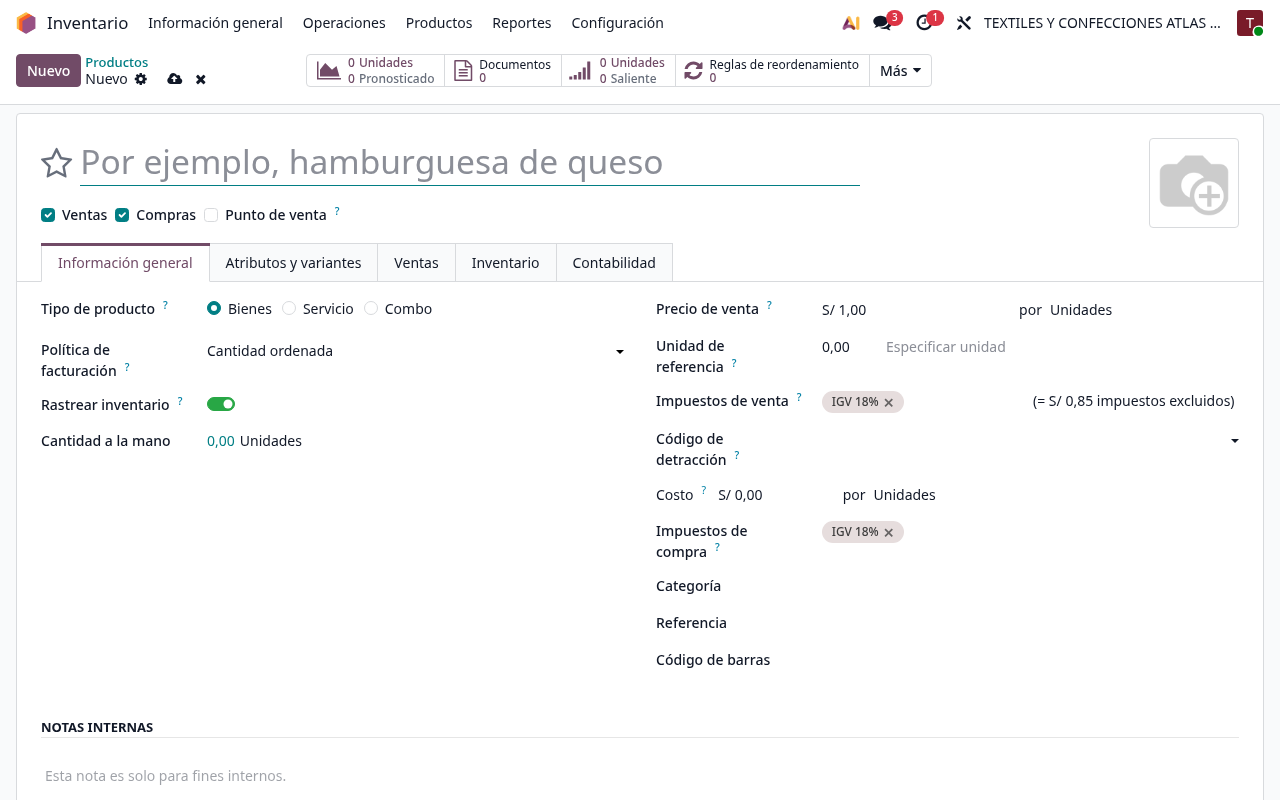
\includegraphics[width=1.15\textwidth]{images/inventario_crud_fill_name.png}}
\end{center}
\begin{center}
    \makebox[\textwidth][c]{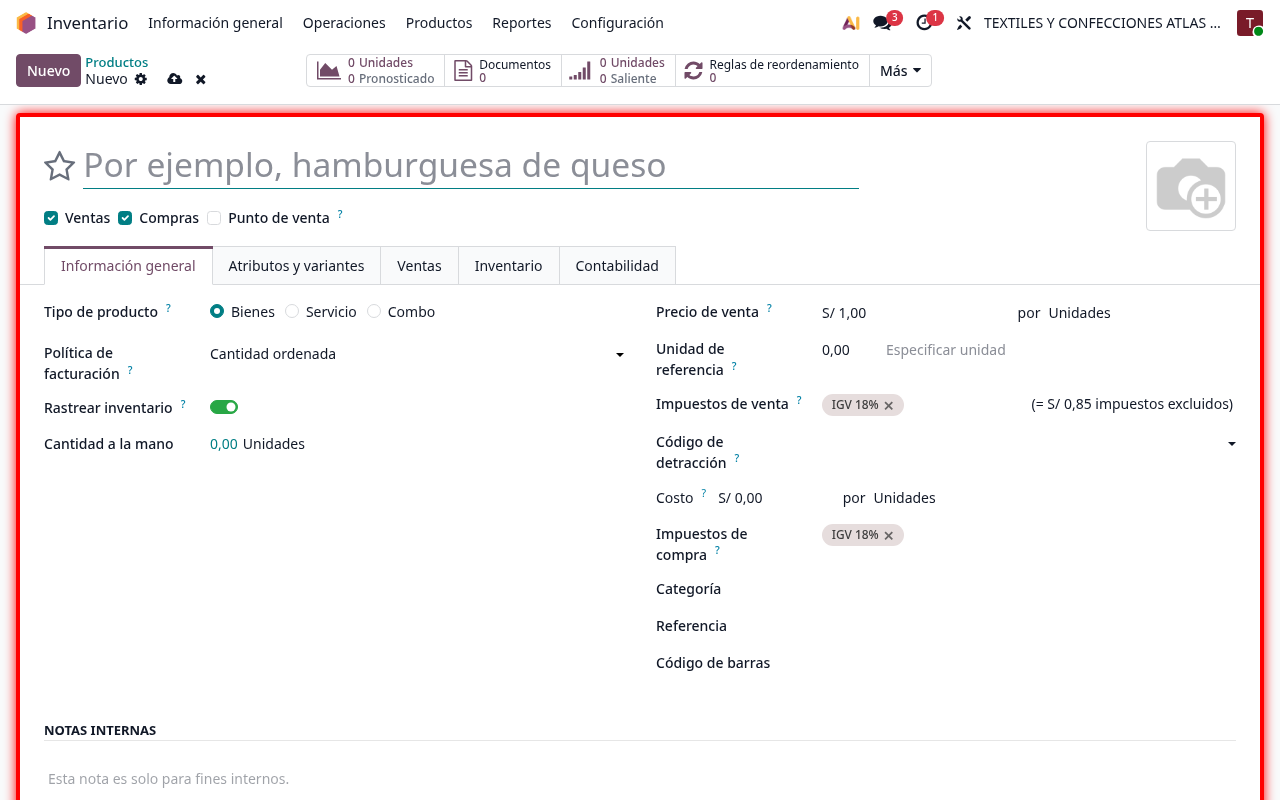
\includegraphics[width=1.15\textwidth]{images/inventario_crud_fill_type.png}}
\end{center}
\newpage

\section{Módulo de Punto de Venta (PoS - Operaciones de Caja)}
Este es el módulo que utilizarás para vender rápido cara a cara al cliente en mostrador.

\subsection{Abrir la Caja del Día}
\begin{enumerate}
    \item Haz clic en el módulo \textbf{Punto de Venta}.
    \item Ubica tu caja y haz clic en el botón \textbf{Nueva Sesión} o \textbf{Continuar} (enmarcado en rojo).
\end{enumerate}

\begin{center}
    \makebox[\textwidth][c]{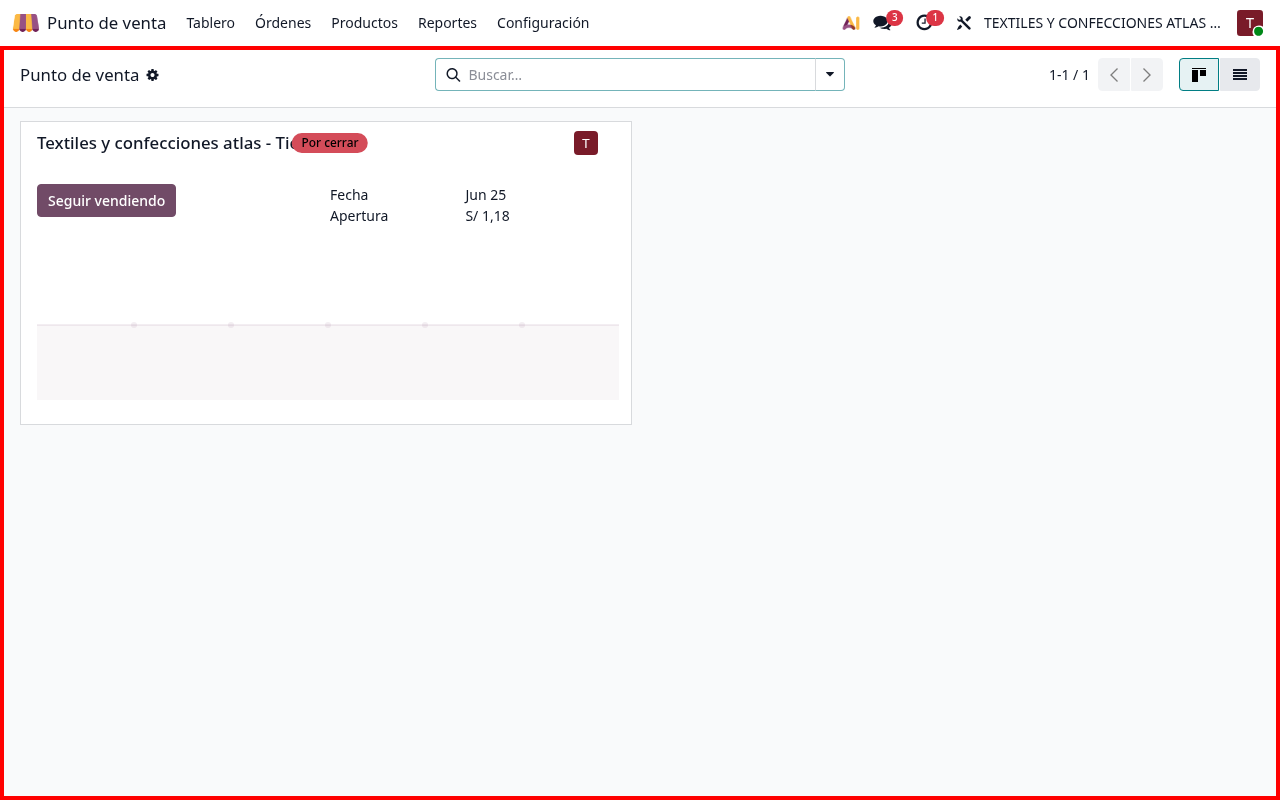
\includegraphics[width=1.15\textwidth]{images/pos_crud_read.png}}
\end{center}
\begin{center}
    \makebox[\textwidth][c]{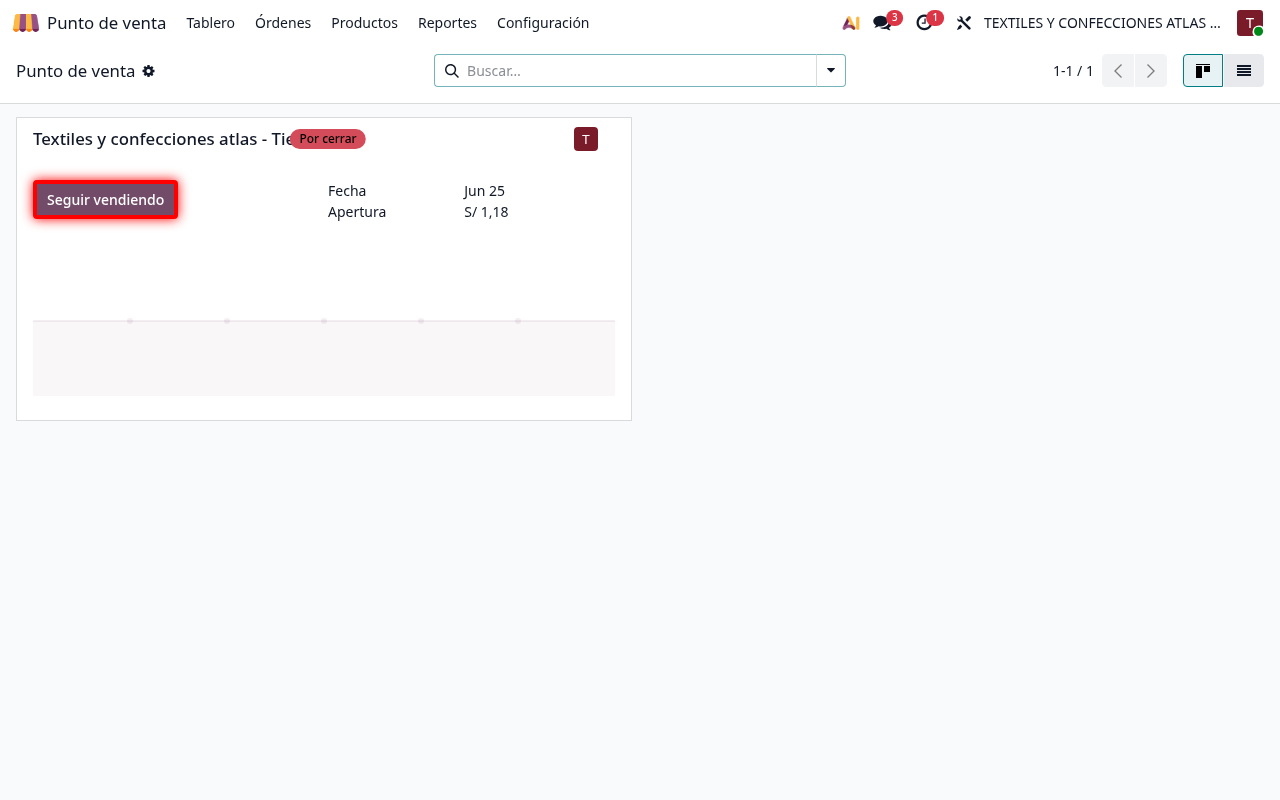
\includegraphics[width=1.15\textwidth]{images/pos_click_nueva_sesion.png}}
\end{center}

\subsection{Cobro y emisión de Boleta/Factura}
\begin{enumerate}
    \item Haz clic sobre los productos a vender para cargarlos al carrito izquierdo.
    \item Haz clic en el botón verde grande que dice \textbf{Pago}.
    \item Elige el \textbf{Método de Pago} (Efectivo o Tarjeta).
    \item Elige a la derecha si deseas emitir una \textbf{Factura} (obligatorio tener RUC del cliente) o \textbf{Boleta/Recibo}.
    \item Haz clic en \textbf{Validar} para finalizar la venta e imprimir.
\end{enumerate}
\newpage

\section{Módulo de Ventas B2B (Cotizaciones Mayoristas)}
Se usa para pedidos grandes o ventas corporativas donde el cliente solicita un presupuesto formal antes de pagar.

\subsection{Ver Historial de Ventas}
\begin{enumerate}
    \item Haz clic en el módulo \textbf{Ventas}.
    \item Verás la lista de cotizaciones existentes y su estado (Borrador, Confirmado).
\end{enumerate}

\begin{center}
    \makebox[\textwidth][c]{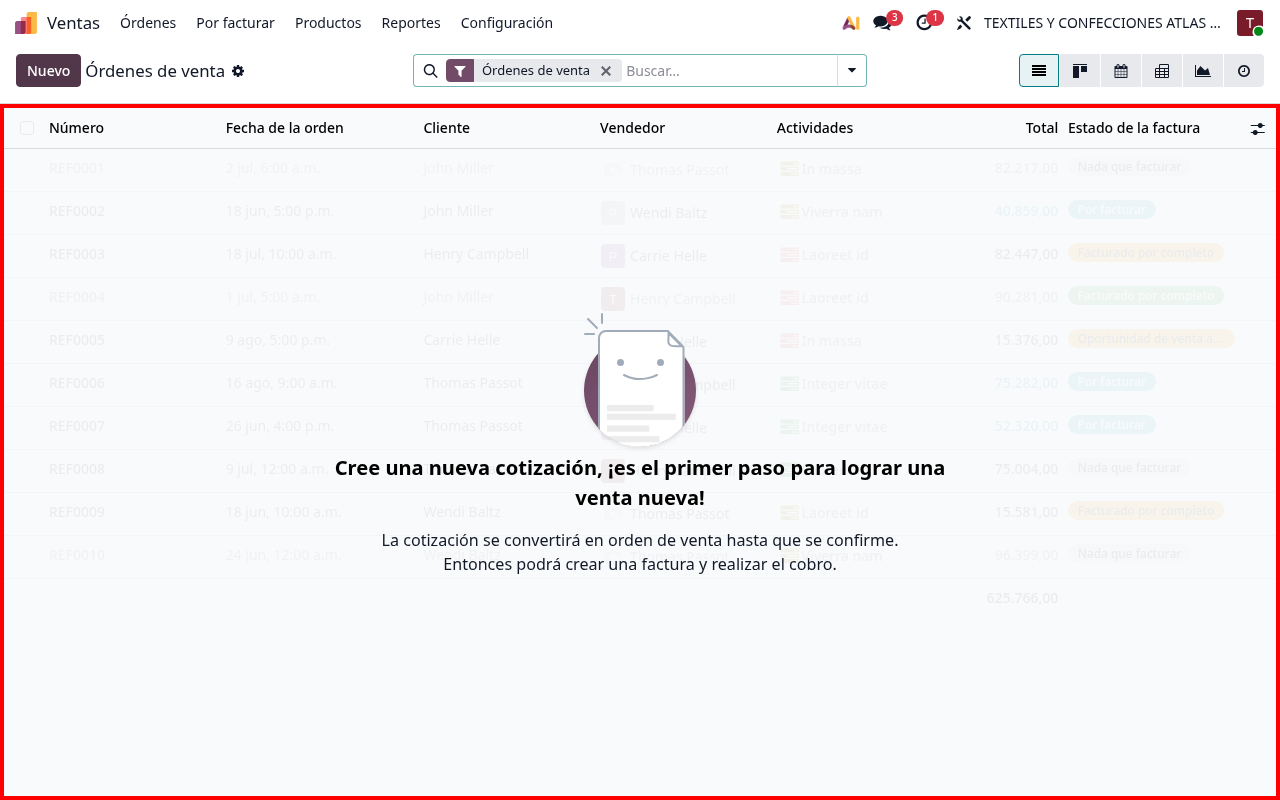
\includegraphics[width=1.15\textwidth]{images/ventas_crud_read.png}}
\end{center}

\subsection{Crear una Cotización de Venta (Ejemplo Práctico)}
\begin{enumerate}
    \item Haz clic en \textbf{Nuevo} arriba a la izquierda.
    \item Selecciona al \textbf{Cliente} de la lista desplegable.
    \item En la sección de abajo, haz clic en \textbf{Agregar un producto} y selecciona la prenda y la cantidad (Ejemplo: 50 unidades de \textit{Casaca Térmica Impermeable Talla L}).
    \item Haz clic en \textbf{Confirmar} para concretar el pedido de venta.
\end{enumerate}

\begin{center}
    \makebox[\textwidth][c]{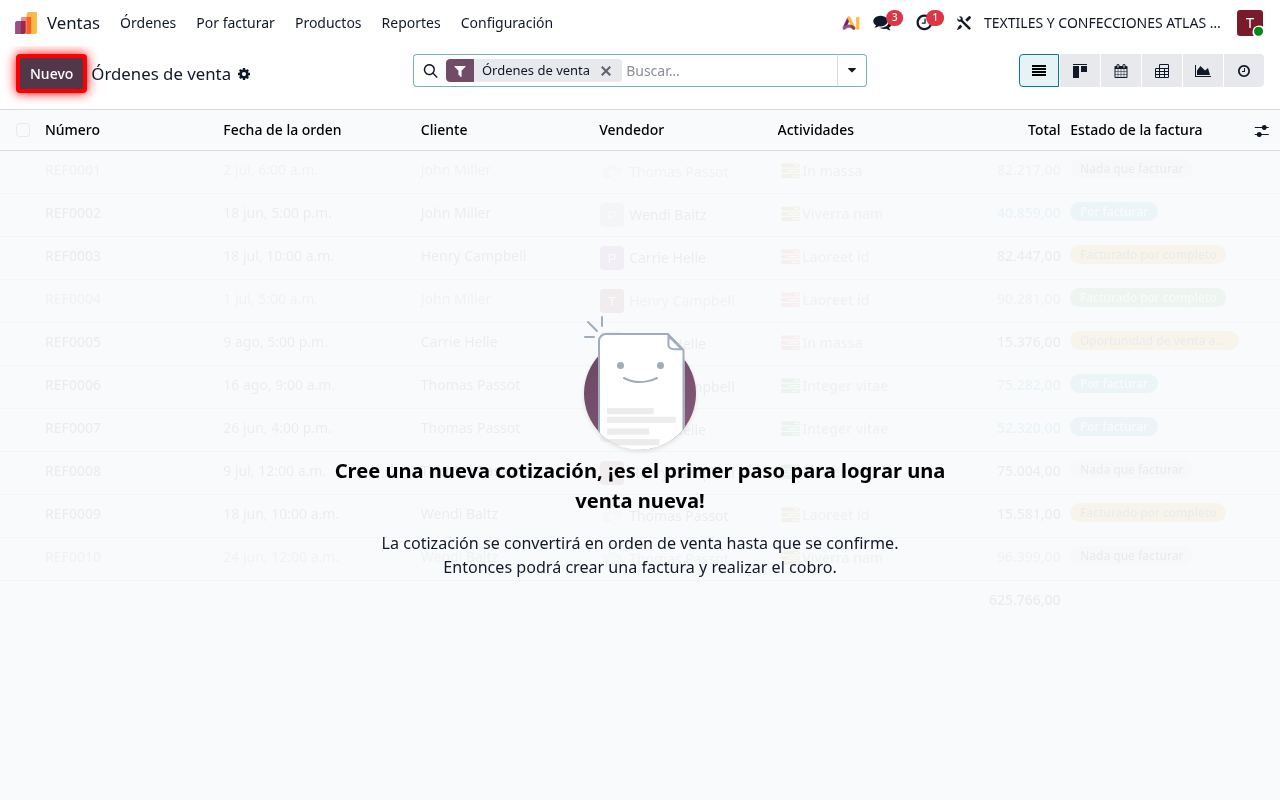
\includegraphics[width=1.15\textwidth]{images/ventas_crud_click_create.png}}
\end{center}
\begin{center}
    \makebox[\textwidth][c]{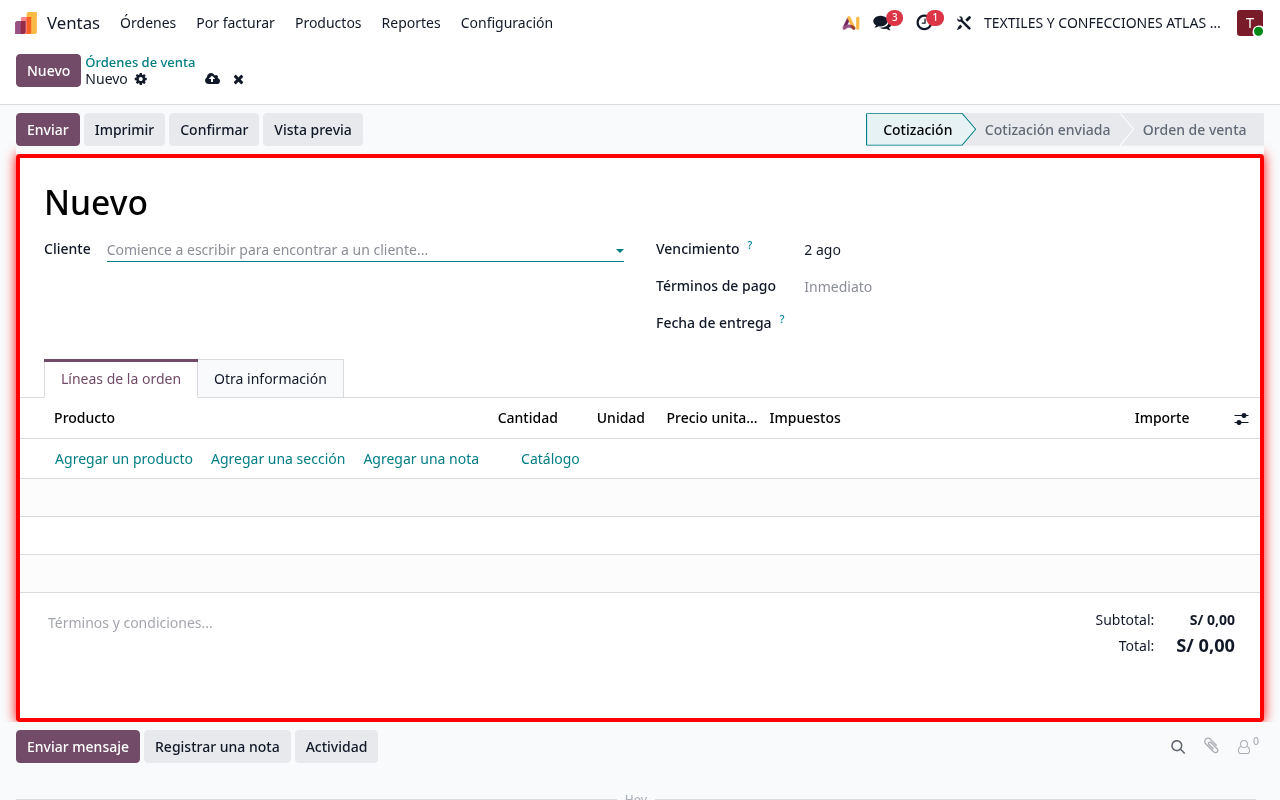
\includegraphics[width=1.15\textwidth]{images/ventas_crud_form.png}}
\end{center}
\newpage

\end{document}
